% This is text associated with the open textbook "Open Electromagnetics"
% See immediately below for author, date
% This work is licensed under the Creative Commons Attribution-ShareAlike 4.0 International License. (CC BY SA 4.0) 
% To view a copy of the license, visit http://creativecommons.org/licenses/by-sa/4.0/

%ORB TITLE Boundary Conditions on the Magnetic Field Intensity ({\bf H}) 
%ORB AUTHOR 0        # S.W. Ellingson, Virginia Tech (ellingson@vt.edu)
%ORB DATE 20180630   # yyyymmdd
%ORB ABSTRACT Boundary Conditions on the Magnetic Field Intensity

\label{m0023_Boundary_Conditions_on_H} % <-- Must match name of this file and module directory name.  Don't mess with this!

In homogeneous media, electromagnetic quantities vary smoothly and continuously.
At a boundary between dissimilar media, however, it is possible for electromagnetic quantities to be discontinuous.
Continuities and discontinuities in fields can be described mathematically by \emph{boundary conditions}
\index{boundary conditions}
and used to constrain solutions for fields away from these boundaries.
In this section, we derive boundary conditions on the magnetic field intensity ${\bf H}$.

To begin, consider a region consisting of only two media that meet at a smooth boundary as shown in Figure~\ref{m0023_fBoundary}.
%
\begin{figure}[b!]
\begin{center}
\pdftooltip{{  % note double braces
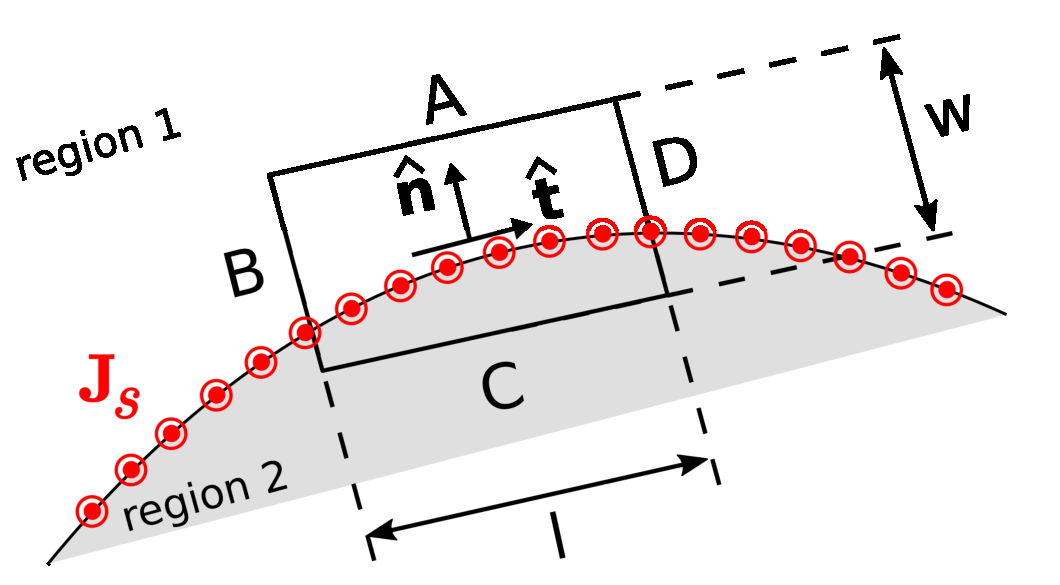
\includegraphics[width=2.5in]{modules/m0023_fBoundary.eps}
}}{A rectangle labeled A, B, C, D (counter-clockwise from the top) centered at a point on a boundary. The long sides of the rectangles are parallel to the surface. The length of the rectangle is l, and the width is w. A vector, t-hat, is tangent to the surface of the boundary. Another vector, n-hat, is perpendicular to the surface of the boundary. On the surface are blue circles with dots in the middle, labeled J sub s. The outer region of the boundary is labeled region 1, and the inner is labeled region 2.}
\end{center} 
% ***WikipediaCommonsURL
%\centerline{\scriptsize 
%\copyright~\hyperref[m0023_fBoundary_Credit]{author} 
%\href{https://creativecommons.org/licenses/by-sa/4.0/}{CC BY~SA 4.0} 
%} 
\caption{
\label{m0023_fBoundary}
Determining the boundary condition on ${\bf H}$ at the smooth boundary between two material regions.
}
\end{figure}
%
The desired boundary condition can be obtained directly from Ampere's Circuital Law (ACL; Section~\ref{m0019_Amperes_Law_Magnetostatics}):
% 
\begin{equation}  
\oint_{\mathcal C}{ {\bf H} \cdot d{\bf l} } = I_{encl}
\label{m0023_eACL}
\end{equation}
% 
where ${\mathcal C}$ is any closed path and $I_{encl}$ is the current that flows through the surface bounded by that path in the direction specified by the ``right-hand rule'' 
\index{right-hand rule!Stokes' theorem}
of Stokes' theorem.
Let ${\mathcal C}$ take the form of a rectangle centered on a point on the boundary as shown in Figure~\ref{m0023_fBoundary}, perpendicular to the direction of current flow at that location.
Let the sides $A$, $B$, $C$, and $D$ be perpendicular and parallel to the boundary.  
Let the length of the parallel sides be $l$, and let the length of the perpendicular sides be $w$.  
Now we apply ACL.  
We must integrate in a counter-clockwise direction in order to be consistent with the indicated reference direction for ${\bf J}_s$.
\index{right-hand rule!Stokes' theorem}
Thus:
% 
\begin{align}   
\oint{ {\bf H} \cdot d{\bf l} } &=\int_A{ {\bf H} \cdot d{\bf l} } & \nonumber \\ 
                                &+\int_B{ {\bf H} \cdot d{\bf l} }  & \nonumber \\ 
                                &+\int_C{ {\bf H} \cdot d{\bf l} }  & \nonumber \\
                                &+\int_D{ {\bf H} \cdot d{\bf l} }  &= I_{encl} 
\end{align}
%  
Now we let $w$ and $l$ become vanishingly small while (1) maintaining the ratio $l/w$ and (2) keeping $\mathcal{C}$ centered on the boundary.
In this process, the contributions from the $B$ and $D$ segments become equal in magnitude but opposite in sign; i.e., 
% 
\begin{equation}   
\int_B{ {\bf H} \cdot d{\bf l} } 
+\int_D{ {\bf H} \cdot d{\bf l} }
\to 0
\end{equation}
%
This leaves
% 
\begin{equation}   
\int_A{ {\bf H} \cdot d{\bf l} } 
+\int_C{ {\bf H} \cdot d{\bf l} }
\to I_{encl}
\end{equation}
%
Let us define the unit vector $\hat{\bf t}$ (``tangent'') as shown in Figure~\ref{m0023_fBoundary}.
Now we have simply: 
% 
\begin{equation}   
  {\bf H}_1 \cdot \left(-\hat{\bf t}\Delta l\right)
+ {\bf H}_2 \cdot \left(+\hat{\bf t}\Delta l\right) 
= I_{encl} 
\label{m0023_eACL2}
\end{equation}
%
where ${\bf H}_1$ and ${\bf H}_2$ are the fields evaluated on the two sides of the boundary, and
$\Delta l \to 0$ is the length of sides $A$ and $C$.
As always, $I_{encl}$ (units of A) may be interpreted as the flux
\index{flux}
of the current density ${\bf J}_s$ (units of A/m) flowing past a line on the surface having length $\Delta l$ (units of m) perpendicular to $\hat{\bf t}\times\hat{\bf n}$, where $\hat{\bf n}$ is the normal to the surface, pointing into Region~1.  Stated mathematically:
%
\begin{equation}
I_{encl} \rightarrow {\bf J}_s \cdot \left( \Delta l ~ \hat{\bf t}\times\hat{\bf n} \right)
\end{equation}
% 
Before proceeding, note this is true regardless of the particular direction we selected for $\hat{\bf t}$; it is only necessary that $\hat{\bf t}$ be tangent to the boundary. Thus, $\hat{\bf t}\times\hat{\bf n}$ need not necessarily be in the same direction as ${\bf J}_s$.
%
Now Equation~\ref{m0023_eACL2} can be written:
% 
\begin{equation}   
  {\bf H}_2 \cdot       \hat{\bf t}                        \Delta l
- {\bf H}_1 \cdot       \hat{\bf t}                        \Delta l 
= {\bf J}_s \cdot \left(\hat{\bf t}\times\hat{\bf n}\right)\Delta l
\end{equation}
%
Eliminating the common factor of $\Delta l$ and arranging terms on the left:
% 
\begin{equation}   
 \left( {\bf H}_2 -{\bf H}_1 \right) \cdot \hat{\bf t} = {\bf J}_s \cdot \left(\hat{\bf t}\times\hat{\bf n}\right)
\label{m0023_eACL3}
\end{equation}
%
The right side may be transformed using a vector identity (Equation~\ref{m0140_eVI1} of Section~\ref{m0140_Vector_Identities}) to obtain:
% 
\begin{equation}   
\left( {\bf H}_2 -{\bf H}_1 \right) \cdot \hat{\bf t} = \hat{\bf t} \cdot \left( \hat{\bf n} \times {\bf J}_s \right)
\label{m0023_eBC1}
\end{equation}
%
%Now recall our earlier statement about the direction of $\hat{\bf t}$.
%; in other words, this must be true for \emph{any} unit vector that is tangent to the surface, and not just for $\hat{\bf t}$ directed as shown in Figure~\ref{m0023_fBoundary}.
Equation~\ref{m0023_eBC1} is the boundary condition we seek.  
We have found that the component of ${\bf H}_2 -{\bf H}_1$ (the difference between the magnetic field intensities at the boundary) in any direction tangent to the boundary is equal to the component of the current density flowing in the perpendicular direction $\hat{\bf n} \times {\bf J}_s$.  Said differently: 
%
%ORB HIGHLIGHT
\begin{mdframed}[backgroundcolor=yellow!20,nobreak=true] 
A discontinuity in the tangential component of the magnetic field intensity at the boundary must be supported by surface current flowing in a direction perpendicular to this component of the field.
\end{mdframed}
%
An important consequence is that:
%
%ORB HIGHLIGHT
\begin{mdframed}[backgroundcolor=yellow!20,nobreak=true] 
If there is no surface current, then the tangential component of the magnetic field intensity is continuous across the boundary.
\end{mdframed}

It is possible to obtain a mathematical form of the boundary condition that is more concise and often more useful than Equation~\ref{m0023_eBC1}.
This form may be obtained as follows.
First, we note that the dot product with respect to $\hat{\bf t}$ on both sides of Equation~\ref{m0023_eBC1} means simply ``any component that is tangent to the boundary.''  We need merely to make sure we are comparing the same tangential component on each side of the equation.  
For example $\hat{\bf n} \times \left( {\bf H}_2 -{\bf H}_1 \right)$ is tangential to the boundary, since $\hat{\bf n}$ is perpendicular to the boundary and therefore any cross product involving $\hat{\bf n}$ will be perpendicular to $\hat{\bf n}$.
The corresponding component of the current density is $\hat{\bf n} \times \left( \hat{\bf n} \times {\bf J}_s \right)$, so Equation~\ref{m0023_eBC1} may be equivalently written as follows: 
% 
\begin{equation}   
\hat{\bf n} \times \left( {\bf H}_2 -{\bf H}_1 \right)  = \hat{\bf n} \times \hat{\bf n} \times {\bf J}_s 
\label{m0023_eBC2}
\end{equation}
%
Applying a vector identity (Equation~\ref{m0140_eVI2} of Section~\ref{m0140_Vector_Identities}) to the right side of Equation~\ref{m0023_eBC2} we obtain: 
%
\begin{align}   
\hat{\bf n} \times \hat{\bf n} \times {\bf J}_s 
     &= \hat{\bf n} \left(\hat{\bf n}\cdot{\bf J}_s\right) - {\bf J}_s\left(\hat{\bf n}\cdot\hat{\bf n}\right) \nonumber \\
     &= \hat{\bf n} \left(0\right) - {\bf J}_s\left(1\right) \nonumber \\
     &= -{\bf J}_s
\end{align}
%
Therefore:
% 
\begin{equation}   
\hat{\bf n} \times \left( {\bf H}_2 -{\bf H}_1 \right)  = -{\bf J}_s
\end{equation}
%
The minus sign on the right can be eliminated by swapping ${\bf H}_2$ and ${\bf H}_1$ on the left, yielding
% 
\begin{equation}   
\boxed{
 \hat{\bf n} \times \left( {\bf H}_1 -{\bf H}_2 \right) = {\bf J}_s                                              
}
\end{equation}
%
This is the form in which the boundary condition is most commonly expressed.

It is worth noting what this means for the magnetic field intensity ${\bf B}$. Since ${\bf B}=\mu{\bf H}$:
%
%ORB HIGHLIGHT
\begin{mdframed}[backgroundcolor=yellow!20,nobreak=true] 
In the absence of surface current, the tangential component of ${\bf B}$ across the boundary between two material regions is discontinuous if the permeabilities are unequal.
\end{mdframed}

